\documentclass[12pt, a4paper]{article}

\usepackage{array}
\usepackage[portuguese]{babel}
\usepackage{chngpage}
\usepackage{float}
\usepackage[a4paper, margin=2cm]{geometry}
\usepackage{graphicx}
\usepackage{hyperref}
\usepackage{setspace}
\usepackage{xcolor}

\title{\Huge \textbf{Computação Gráfica \\ \Large Trabalho Prático -- Fase I}}
\date{2 de março 2025}
\author{Grupo \textbf{\color{red} TODO}}

\begin{document}

\begin{center}
    
\includegraphics[width=0.25\textwidth]{res/cover/EE-C.eps}
\end{center}

\chardef\_=`_
\onehalfspacing
\setlength{\parskip}{\baselineskip}
\setlength{\parindent}{0pt}
\def\arraystretch{1.5}

{\let\newpage\relax\maketitle}
\maketitle
\thispagestyle{empty}

\vspace*{\fill}

\begin{adjustwidth}{-2cm}{-2cm} % These values only need to be large enough to center the table
    \begin{center}
        \begin{tabular}{>{\centering}p{0.25\textwidth}
                        >{\centering}p{0.25\textwidth}
                        >{\centering}p{0.25\textwidth}
                        >{\centering\arraybackslash}p{0.25\textwidth}}
            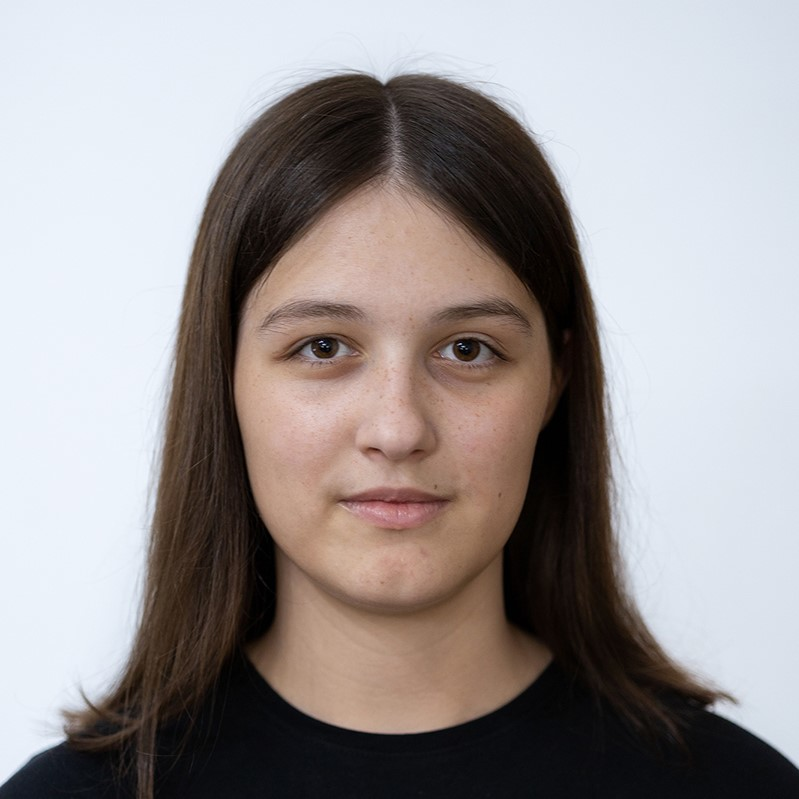
\includegraphics[width=3.5cm]{res/cover/A104437.png} &
            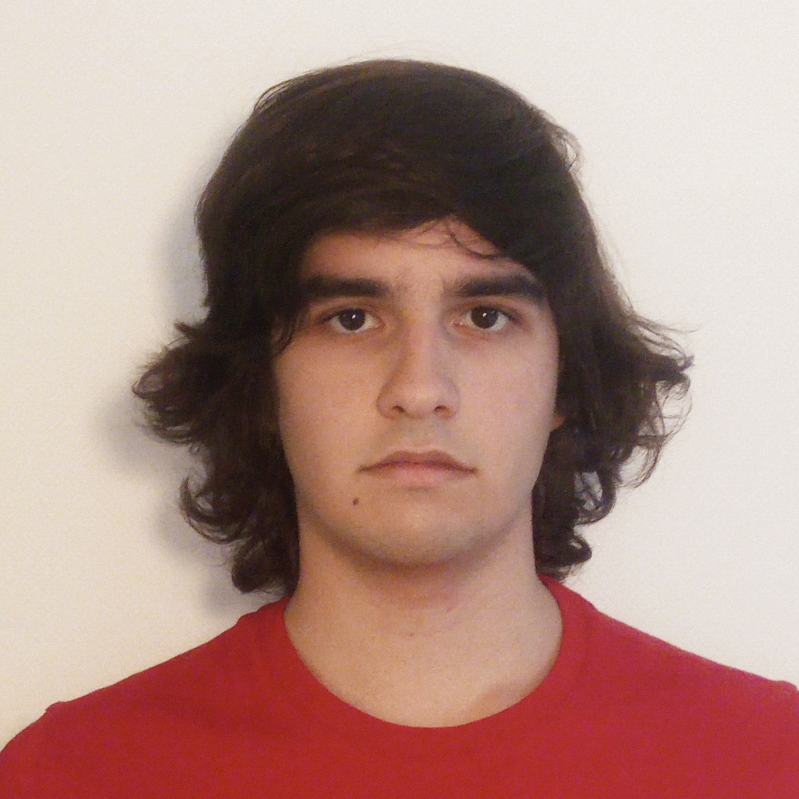
\includegraphics[width=3.5cm]{res/cover/A104348.png} &
            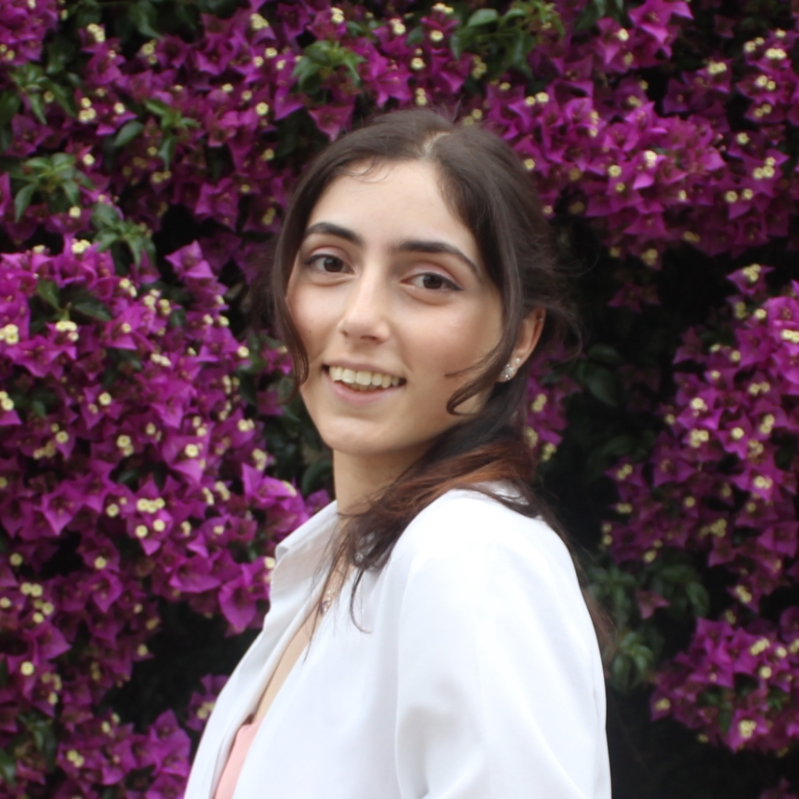
\includegraphics[width=3.5cm]{res/cover/A90817.png} &
            
\includegraphics[width=3.5cm]{res/cover/A104179.png} \\

            Ana Oliveira & Humberto Gomes & Mariana Cristino & Sara Lopes \\
            A104437      & A104348        & A90817           & A104179
        \end{tabular}
    \end{center}
\end{adjustwidth}

\pagebreak

\begin{abstract}
    \textbf{\color{red} TODO - resumo}
\end{abstract}

\section{\emph{Generator}}

\textbf{\color{red} TODO - \emph{generator}}

\section{\emph{Engine}}

\textbf{\color{red} TODO - \emph{engine}}

\subsection{Câmara}

A câmara é responsável por definir a perspetiva e o enquadramento da cena 3D. A sua configuração
segue um modelo de câmara em primeira pessoa, com a posição, orientação e projeção definidas a
partir do ficheiro XML da cena.

A posição da câmara é representada pelo vetor \texttt{position}, que define a sua localização no
espaço tridimensional. A direção para onde a câmara está orientada é determinada pelo vetor
\texttt{lookAt}, um ponto no espaço para onde a lente da câmara aponta. O vetor \texttt{up}
especifica a orientação vertical da câmara, garantindo a sua correta rotação no espaço. Estes três
vetores são utilizados para calcular a matriz de visualização.

Uma vez que este projeto usa \emph{shaders}, não é possível utilizar a função \texttt{gluLookAt}
\cite{gluLookAt}, usada nas aulas práticas para o cálculo da matriz de visualização. No entanto,
como utilizamos a biblioteca \texttt{glm} \cite{glm}, é usada a função equivalente
\texttt{glm::lookAt}, que devolve uma matriz que pode ser passada ao \emph{shader} de vértices.

A projeção da câmara é controlada pelo campo de visão (\emph{Field of View} -- FOV) e pelos planos
de recorte próximo e distante (\texttt{near} e \texttt{far}). O FOV define o ângulo de abertura da
câmara, influenciando a sensação de profundidade da cena, enquanto os planos de recorte estabelecem
os limites mínimo e máximo da região visível. A matriz de projeção é calculada com a função
\texttt{glm::perspective}, que utiliza o $FOV$, o \emph{aspect ratio} da janela, e os planos de
recorte para definir a forma como os objetos são projetados no espaço 3D.

A matriz final da câmara resulta da multiplicação da matriz de projeção pela matriz de visualização,
e é atualizada sempre que a janela é redimensionada. É utilizada para transformar todos os objetos
da cena, garantindo um enquadramento adequado dos mesmos e a renderização correta da cena.

De momento, a \texttt{engine} não suporta que o utilizador controle a posição da câmara
dinamicamente, movendo-a após a leitura do ficheiro XML. No entanto, pretendemos implementar esta
funcionalidade na segunda fase do projeto.

\section{Resultados obtidos}

\textbf{\color{red} TODO - resultados}

\section{Conclusão e Trabalho Futuro}

\textbf{\color{red} TODO - conclusão}

\begingroup
\section{Bibliografia}
\renewcommand{\section}[2]{}

\begin{thebibliography}{9}
    \bibitem{gluLookAt}
        "gluLookAt."{} Khronos Registry. Accessed: Mar. 2, 2025. [Online.] Available:
        \url{https://registry.khronos.org/OpenGL-Refpages/gl2.1/xhtml/gluLookAt.xml}
    \bibitem{glm}
        "glm."{} GitHub. Accessed: Mar. 2, 2025. [Online.] Available:
        \url{https://github.com/g-truc/glm}
    \bibitem{exemplo}
        \href{https://youtu.be/dQw4w9WgXcQ}{Um item de exemplo na bibliografia}
\end{thebibliography}
\endgroup

\end{document}
